% !TEX root = ../literature.tex
\subsection{Public space and cross-device natural user interaction}
Different field of studies have long held the view that the physical and social dynamics of public space play a central role in the formation of publics and public culture. Car et al, argued \emph{"when public spaces are successful [...] they will increase opportunities to participate in communal activity. This fellowship in the open nurtures the growth of public life, which is stunted by the social isolation."} \cite{carr:1992}. For Computer Science this view was embraced with the new opportunities presented by the technological possibility to include the public space inside the ecology of a computer system. As such research investigating how public space can affect interaction with the system and vice versa spanned.

In historical perspective Brignull and Rogers work\cite{Brignull:2003} is the first that investigates interaction flow in the context of public space for large displays. They observe that even though large displays are increasingly placed in public places, to support community and social activities, people are reluctant to use them. They point out that the main reason, for existing resistance by the public to participate, is the prominence of the affective aspect of the  user experience - feelings of social embarrassment. In order to understand this phenomenon they create a conceptual framework for analyzing public interaction. Their framework consist of three different spaces (1) Space A peripheral awareness of displays - people are engage in unrelated activities (2) Space B focal awareness - - people are engage in associated activities (3) Space C direct interaction - people engage in interaction with the display. They point out \emph{" it appears that the key bottlenecks occurs in public interaction when people have to make transitions between different activity spaces "}. They conclude  it is crucial for public interaction to be able seamlessly and comfortably to transition between onlooker and participant and one way to do that is to encourage people to cross the thresholds from peripheral awareness to focal awareness without becoming self-conscious.

While Brignull and Rogers work focuses on interaction with Large Displays, Cheung et al.  extends that to interaction barriers for cross-device public displays \cite{Cheung:2014}. They focus on interaction process comprised of personal devices (capturing unique traits such as privacy and novel interaction mechanisms), and a large display (which is used as a shared display, and a direct input alternative, if supported), and list in partial order the usage barriers, for engaging a passerby while clustering them in three groups: (1) Attract - how can we combat display blindness (notice the display), interaction blindness (be aware we can interact with the display), and cross-device blindness (be aware we can use personal devices as a mean of interaction); (2) Interact - how can we combat complex interaction (easily understand how to make use of large display and personal device), social inhibition (do not feel social embarrassment),  and how can we opt-in/out (engage or withdraw from the system); (3) Manage - how can we maintain and communicate the connection between the large display and personal device (connecting, explicit disconnecting, implicit disconnecting), how can we recover from interrupting states (eg. Phonecall). After identifying the barriers to cross - device interaction \Cref{fig:111} they model the interaction process as a series of states \Cref{fig:222} stating that ideally a passerby will proceed through each state and engage the system. They conclude that each barrier in their design framework must be addressed in order for the users to be enticed to interact with the system.


\begin{figure}[H]
	\centering
	\subfloat[]{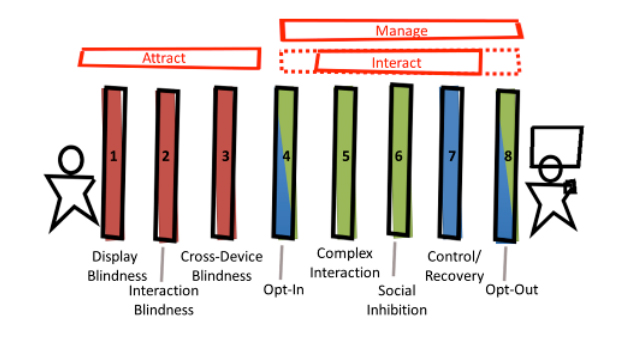
\includegraphics[width = 1\columnwidth , height = 4cm ]{images/111.jpg}\label{fig:111}}\\ 
	\subfloat[]{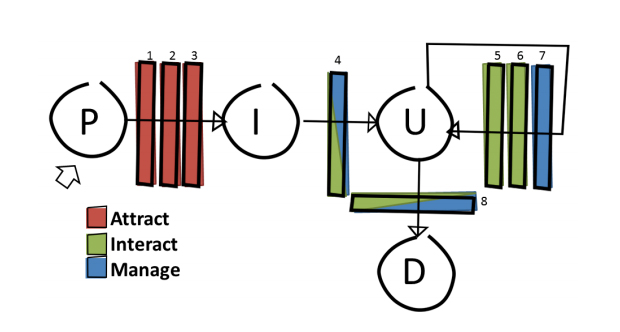
\includegraphics[width = 1\columnwidth , height = 4cm ]{images/222.jpg}\label{fig:222}}
	\caption{
		Adopted from Cheung et al. \protect\cite{Cheung:2014}.
		\protect\subref{fig:111} cross-device interaction barriers for interacting with large displays and hand-held device
		\protect\subref{fig:222} States  of interaction and barriers encountered.(P:Passing, I:Interested, U:Using, D:Done).
		}
	\label{fig:Cheung et al. ideas}
\end{figure}

To summarize there is a need to take physical and social dynamics into consideration when designing for public space as people are reluctant to use public installations. Car et al. argues that opportunities to participate in communal activity are increased when public spaces are successful, which in turn nurtures the growth of public life \protect\cite{carr:1992}. Brignull, Rogers \protect\cite{Brignull:2003}, and Cheung et al. \protect\cite{Cheung:2014} all agrees that people avoid the installations due to social inhibition. Brignull and Rogers creates a conceptual framework for analyzing public interaction and trying to understand why people feel social embarrassment. They argue that the key bottleneck in public interaction occurs when people have to transits between activity spaces and concludes that it is necessary that people can comfortably and seamlessly transit between being an onlooker and a participant. They suggest to encourage the people to make the transition while avoiding that they become self-conscious about it. .

Cheung et al. tries to identify and list the usage barriers for engaging a passerby into interaction between a public display and their personal device. They identify 3 groups of barriers: (1) Attraction - how can we make people notice the display and realize that they can interact with it? (2) Interact - How can we make a system that is easy for the people to understand and use without feeling socially embarrassed? And (3) Manage - How can we maintain and avoid interruptions in communication between the public display and the peoples personal device.
They make a model that describe the barriers and conclude that those barriers must be addressed for making people interested in interacting with the system.

While there are challenges to overcome in the public space, we also saw research that suggested improvement of the usability of the system. When it comes to interacting with public displays, Walter et al. \protect\cite{Walter:2014} points out that many public displays today only show content that cannot be interacted with. They suggest that public displays would benefit from techniques for interacting with its content and make the platform of interactive public display more attractive to users. They derived 4 techniques from lab studies and verified their usability in a field study, which they suggest for interacting with public displays. 
In the field of Cross-Device Interaction Rikimoto \protect\cite{Rekimoto:1997} suggest a pick-and-drop technique for data transfer between devices. He argues that the technique does not does not differ from the traditional remote copy command, but that the added layer of physicalness makes a difference for the user. He states that we live in a fusion of the physical (real) and virtual (computer) world, and the reason to select a technique that adds physicalness to the user interface is because traditional data transfer are too virtual and hard to learn without physical aspects.

 These findings carry the notion that there is a need to investigate the fusion of cross-device interaction and natural user interaction fields in public space context. %Team HCI  F yeah coming to save your digital life yeah! Team HCI F yeah, Science is the only way yeah!  
%It's the dream that we all share, It's the hope for tomorrow, F yeah! 

